\chapter{Zaman Domeni Kriterleri}
Sürekli zamanda tanımlı birinci dereceden bir transfer fonksiyonu
\begin{equation}
    G(s)=\frac{p}{s+p}\label{eqn:1storder_sys}
\end{equation}
olarak verilsin. Birim basamak giriş için yanıt
\begin{equation}
\begin{split}
    y(t)&=\mathcal{L}^{-1}\left\{\frac{p}{s+p}\cdot\frac{1}{s}\right\}\\
    &=\mathcal{L}^{-1}\left\{\frac{1}{s}\right\}-\mathcal{L}^{-1}\left\{\frac{1}{s+p}\right\}\\
    &=1-e^{-pt}
\end{split}
\end{equation}
şeklinde hesaplanır. $e^{-t}$ fonksiyonunun aldığı değerler için Çizelge~\ref{tbl:exp_func} verilmiştir.
% \setlength{\tabcolsep}{40pt}
\begin{table}[!htb]
    \centering
    \caption{$e^{-t}$ fonksiyonunun aldığı değerler}
    \label{tbl:exp_func}
    \begin{tabularx}{\textwidth}{ccc}\hline
        Zaman $t(s)$& Değer $e^{-t}$& $1-e^{-t}$\\[5pt]\hline
        $1$& $0.3679$& $0.6321$\\[5pt]
        $2$& $0.1353$& $0.8647$\\[5pt]
        $3$& $0.0498$& $0.9502$\\[5pt]
        $4$& $0.0183$& $0.9817$\\[5pt]
        $5$& $0.0067$& $0.9933$\\[5pt]
        $6$& $0.0025$& $0.9975$\\[5pt]\hline
    \end{tabularx}
\end{table}
Görüldüğü üzere \ref{eqn:1storder_sys} ile verilen sistemin yanıtı $p$ değişkeninin değerinden bağımsız olarak $1$ değerine yakınsamaktadır. $1$ değerini aşmamaktadır. Dolayısıyla aşım değeri $\%0$'dır. Sürekli halde oturduğu değerin $\%2$ altı veya üstü ile tanımlanan $\%2$'lik banda çıkmamak üzere girdiği zamana yerleşme zamanı denir. Bu tanımdan ve Çizelge~\ref{tbl:exp_func}'den yola çıkarak \ref{eqn:1storder_sys} ile verilen sistemin yerleşme zamanı $t_s=4\,s$'dir. $p=1$ olmaması durumunda zaman ekseni genişler veya daralır bu sebepten yerleşme zamanı 
\begin{equation} 
    t_s=\frac{4}{p}
\end{equation} 
ile hesaplanır. İkinci dereceden bir sistem
\begin{equation}
    G(s)=\frac{w_n^2}{s^2+2\zeta w_ns+w_n^2}
\end{equation}
ile tanımlanmaktadır. Burada $\zeta$ sönüm oranı ve $w_n$ doğal frekans olarak adlandırılmaktadır. İkinci dereceden polinomun kökleri bulunurken faydalanılan $\Delta=b^2-4ac$ hesaplanırsa,
\begin{equation}
\begin{split}
    \Delta&=(2\zeta w_n)^2-4 w_n^2\\
    &=4\zeta^2 w_n^2-4 w_n^2\\
    &=4w_n^2(\zeta^2-1)
\end{split}
\end{equation}
elde edilir ve çözümün tipini belirlemek için
\begin{equation}
    \begin{cases}
        \text{gerçel kök}& \Delta>0\quad \zeta>1\\
        \text{çakışık kök}& \Delta=0\quad \zeta=1\\
        \text{karmaşık kök}& \Delta<0\quad 0<\zeta<1
    \end{cases}
\end{equation}
kullanılabilir. $\zeta>1$ durumunda gerçel köklü çözüm olmasından dolayı sistem transfer fonksiyonu
\begin{equation}
    G(s)=\frac{p_1 p_2}{(s+p_1)(s+p_2)}
\end{equation}
olarak güncellenebilir. $p_1>>p_2$ durumunda $p_2$, $p_2>>p_1$ durumunda $p_1$ yanıtın hızını ve davranışını belirler. $\zeta=1$ olması durumunda yanıt birinci dereceden bir sisteme göre daha yavaş olmaktadır. Haricinde, $0<\zeta<1$ durumunda 
\begin{equation} 
    t_s=\frac{4}{\zeta w_n},\quad \text{Aşım}=100\cdot e^{-\frac{\pi\zeta }{\sqrt{1-\zeta^2}}}
\end{equation} 
ile hesaplanmaktadır. İkinci dereceden sistem yanıtı,
\begin{equation}
    y(t)=1-e^{-\zeta w_nt}\left[\cos(\sqrt{1-\zeta^2}w_nt)+\frac{\zeta}{\sqrt{1-\zeta^2}}\sin(\sqrt{1-\zeta^2}w_nt)\right]
\end{equation}
ile ifade edilmektedir. Sinüzoidal terimler salınımlı olduklarından sadece $e^{-\zeta w_nt}$ terimi yerleşme zamanının hesabı için önemlidir ve birinci dereceden sistem ile aynı ifade kullanılmaktadır. Aşım için 
\begin{equation}
\begin{split}
    \frac{dy(t)}{dt}=0\\
    \sin(\sqrt{1-\zeta^2}w_nt^*)(\frac{\zeta}{\sqrt{1-\zeta^2}}-\sqrt{1-\zeta^2}w_n)=0\\
    \sin(\sqrt{1-\zeta^2}w_nt^*)=0\\
    \sqrt{1-\zeta^2}w_nt^*=\pi\\
    t^*=\frac{\pi}{\sqrt{1-\zeta^2}w_n}
\end{split}
\end{equation}
yanıtta yerine yazılırsa
\begin{equation}
    \begin{split}
        M_p&=e^{-\zeta w_nt^*}\left[\cos(\sqrt{1-\zeta^2}w_nt^*)+\frac{\zeta}{\sqrt{1-\zeta^2}}\sin(\sqrt{1-\zeta^2}w_nt^*)\right]\\
        &=e^{-\frac{\pi\zeta }{\sqrt{1-\zeta^2}}}\left[\cos(\pi)+\frac{\zeta}{\sqrt{1-\zeta^2}}\sin(\pi)\right]\\
        &=e^{-\frac{\pi\zeta }{\sqrt{1-\zeta^2}}}
    \end{split}
\end{equation}
elde edilir. Verilen yerleşme zamanı ve aşım formülleri kullanılarak sistem davranışı şekillendirilebilmektedir. Örneğin $t_s=1$ ve aşım $\%10$ olacak şekilde sistem transfer fonksiyonu seçilirse
\begin{equation} 
\begin{split} 
    \zeta&=-\frac{\log(0.1)}{\sqrt{\pi^2+\log(0.1)^2}}=0.591\\
    w_n&=\frac{4}{\zeta t_s}=\frac{4}{0.591}=6.7682
\end{split} 
\end{equation} 
elde edilir. Bu durumda,
\begin{equation} 
    G(s)=\frac{45.81}{s^2+8s+45.81}
\end{equation} 
transfer fonksiyonu elde edilir. 
\begin{enumerate}
    \item 
    \begin{equation}
        G(s)=\frac{p}{s+p}\label{eqn:first_order}
    \end{equation}
    ve $1\leq p\leq 5$ olmak üzere yerleşme zamanı ile sistem kutubu arasındaki ilişkiyi elde ediniz.
    \begin{lstlisting}
    pvec=np.arange(1,5+1,1)
    tsvec=np.zeros(pvec.shape)
    for i in range(0,len(pvec)):
        pval=pvec[i]
        Gs=control.tf(pval,np.array([1,pval]))
        info=control.step_info(Gs)
        tsvec[i]=info['SettlingTime']

    plt.grid('minor')
    plt.xlabel("p")
    plt.ylabel("ts")
    plt.title("p ile ts arasindaki iliski")

    plt.plot(pvec,tsvec,'b')
    plt.show()
    \end{lstlisting}
    \begin{figure}[!htb]
        \centering
        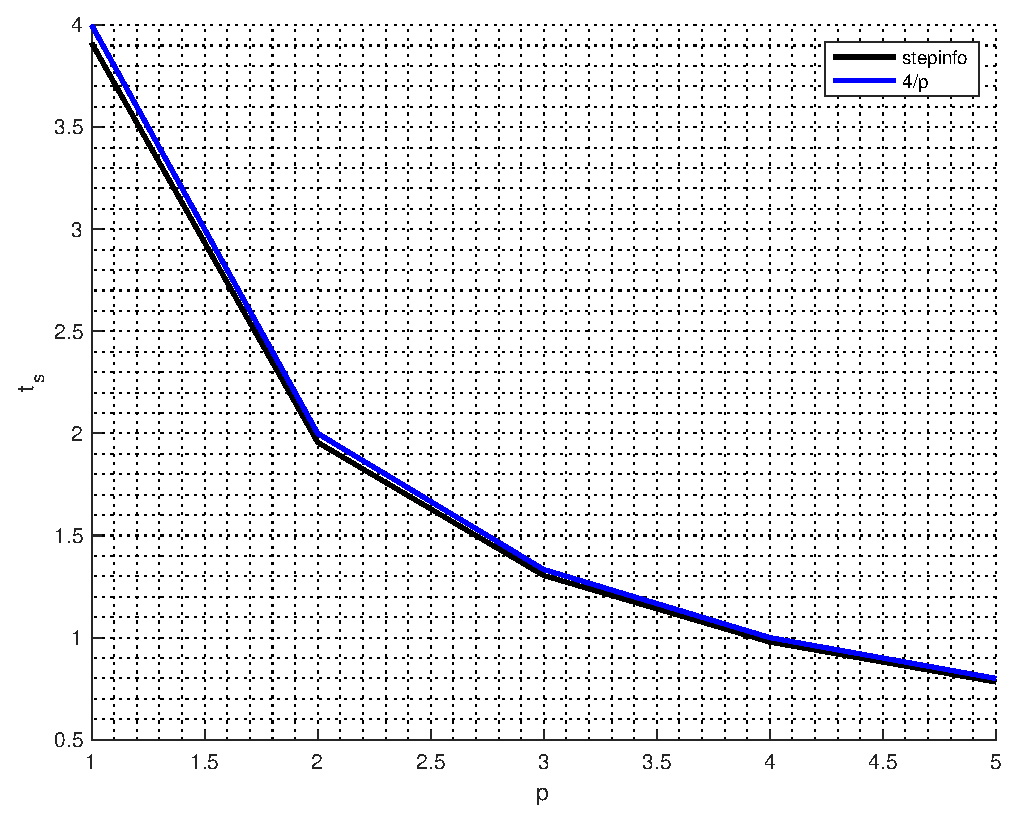
\includegraphics[width=0.5\textwidth]{img/lec4_plot1}
        \caption{Denklem~\ref{eqn:first_order} ile verilen sistem için yerleşme zamanı}
        \label{fig:lec4_plot1}
    \end{figure}
    \item $0<\zeta\leq1$ ve $w_n=2$ olmak üzere 
    \begin{equation}
        G(s)=\frac{w_n^2}{s^2+2\zeta w_ns+w_n^2}
        \label{eqn:second_order}
    \end{equation}
    sisteminin yerleşme zamanının formülünü elde ediniz.
    \begin{lstlisting}
    wn=2
    zetavec=np.arange(0.1,1,0.1)
    tsvec=np.zeros(zetavec.shape)
    tsformula=np.zeros(zetavec.shape)
    for i in range(0,len(zetavec)):
        zetaval=zetavec[i]
        Gs=control.tf(wn**2,np.array([1,2*zetaval*wn,wn**2]))
        info=control.step_info(Gs)
        tsvec[i]=info['SettlingTime']
        tsformula[i]=4/(zetaval*wn)

    plt.grid('minor')
    plt.xlabel("zeta wn")
    plt.ylabel("ts")
    plt.title("zeta wn ile ts arasindaki iliski")


    plt.plot(zetavec*wn,tsformula,'k')
    plt.plot(zetavec*wn,tsvec,'b')
    plt.show()
    \end{lstlisting}
    \begin{figure}[!htb]
        \centering
        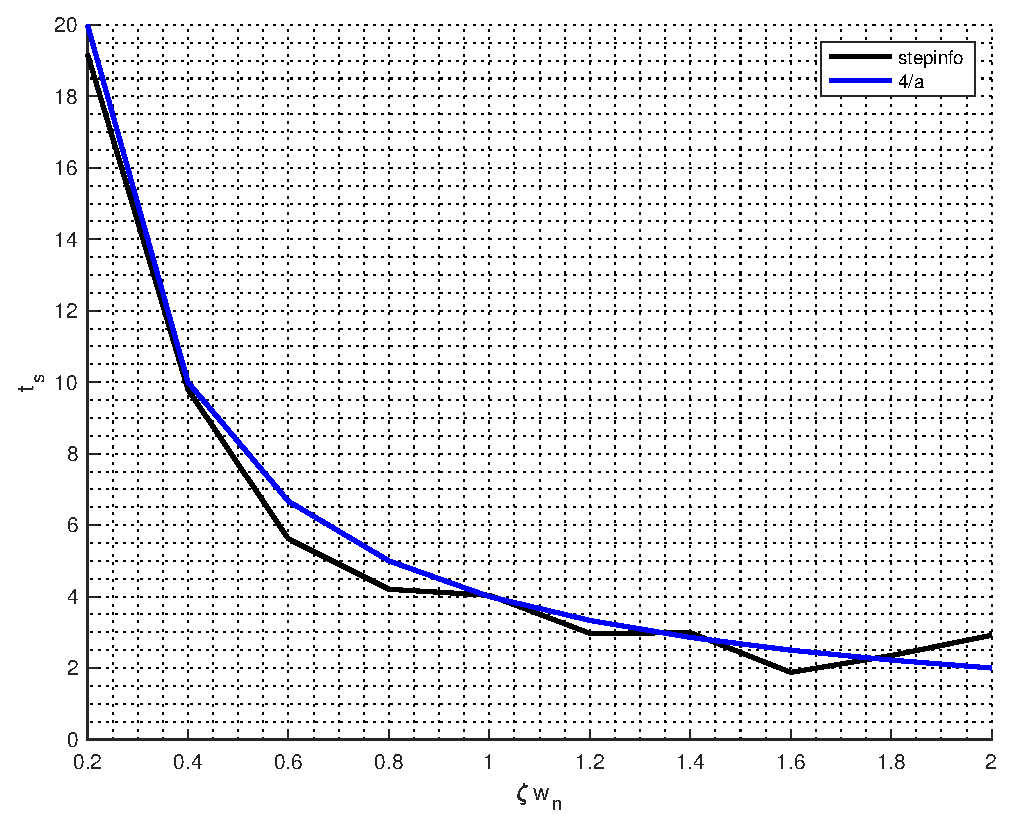
\includegraphics[width=0.5\textwidth]{img/lec4_plot2}
        \caption{Denklem~\ref{eqn:second_order} ile verilen sistem için yerleşme zamanı}
        \label{fig:lec4_plot2}
    \end{figure}
    \item Denklem~\ref{eqn:second_order} sistemi için $1\leq w_n\leq 5$ ve $\zeta=0.6$ değerleri için yerleşme zamanı formülünü elde ediniz.
    \begin{lstlisting}
    zeta=0.6
    wnvec=np.arange(1,5+1,1)
    tsvec=np.zeros(wnvec.shape)
    tsformula=np.zeros(wnvec.shape)
    for i in range(0,len(wnvec)):
        wnval=wnvec[i]
        Gs=control.tf(wnval**2,np.array([1,2*zeta*wnval,wnval**2]))
        info=control.step_info(Gs)
        tsvec[i]=info['SettlingTime']
        tsformula[i]=4/(zeta*wnval)

    plt.grid('minor')
    plt.xlabel("zeta wn")
    plt.ylabel("ts")
    plt.title("zeta wn ile ts arasindaki iliski")


    plt.plot(zeta*wnvec,tsformula,'k')
    plt.plot(zeta*wnvec,tsvec,'b')
    plt.show()
    \end{lstlisting}
    \begin{figure}[!htb]
        \centering
        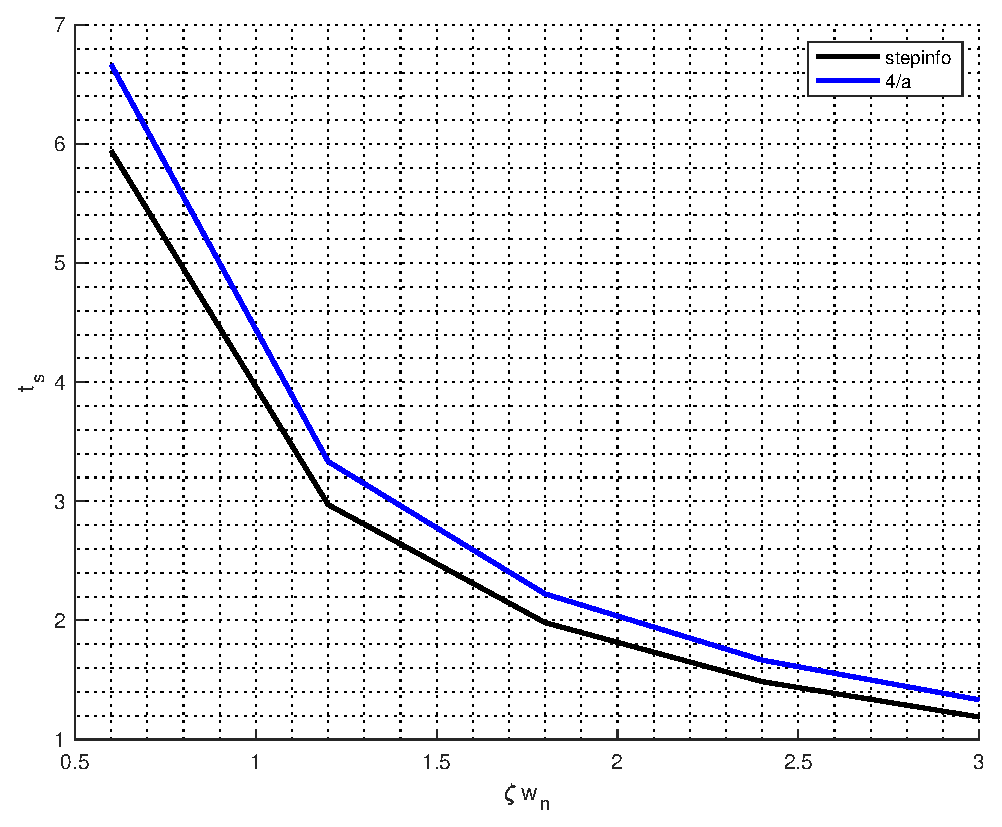
\includegraphics[width=0.5\textwidth]{img/lec4_plot3}
        \caption{Denklem~\ref{eqn:second_order} ile verilen sistem için yerleşme zamanı}
        \label{fig:lec4_plot3}
    \end{figure}
    \item Denklem~\ref{eqn:second_order} sistemi için $0< \zeta<1$ ve $w_n=2$ değerleri için aşımın ifadesini elde ediniz.
    \begin{lstlisting}
    wn=2
    zetavec=np.arange(0.1,1,0.1)
    osvec=np.zeros(zetavec.shape)
    osformula=np.zeros(zetavec.shape)
    for i in range(0,len(zetavec)):
        zetaval=zetavec[i]
        Gs=control.tf(wn**2,np.array([1,2*zetaval*wn,wn**2]))
        info=control.step_info(Gs)
        osvec[i]=info['Overshoot']
        osformula[i]=100*np.exp(-np.pi*zetaval/np.sqrt(1-zetaval**2))

    plt.grid('minor')
    plt.xlabel("zeta")
    plt.ylabel("ts")
    plt.title("zeta ile asim arasindaki iliski")


    plt.plot(zetavec*wn,osformula,'k',linewidth=3)
    plt.plot(zetavec*wn,osvec,'b')
    plt.show()
    \end{lstlisting}
    \begin{figure}[!htb]
        \centering
        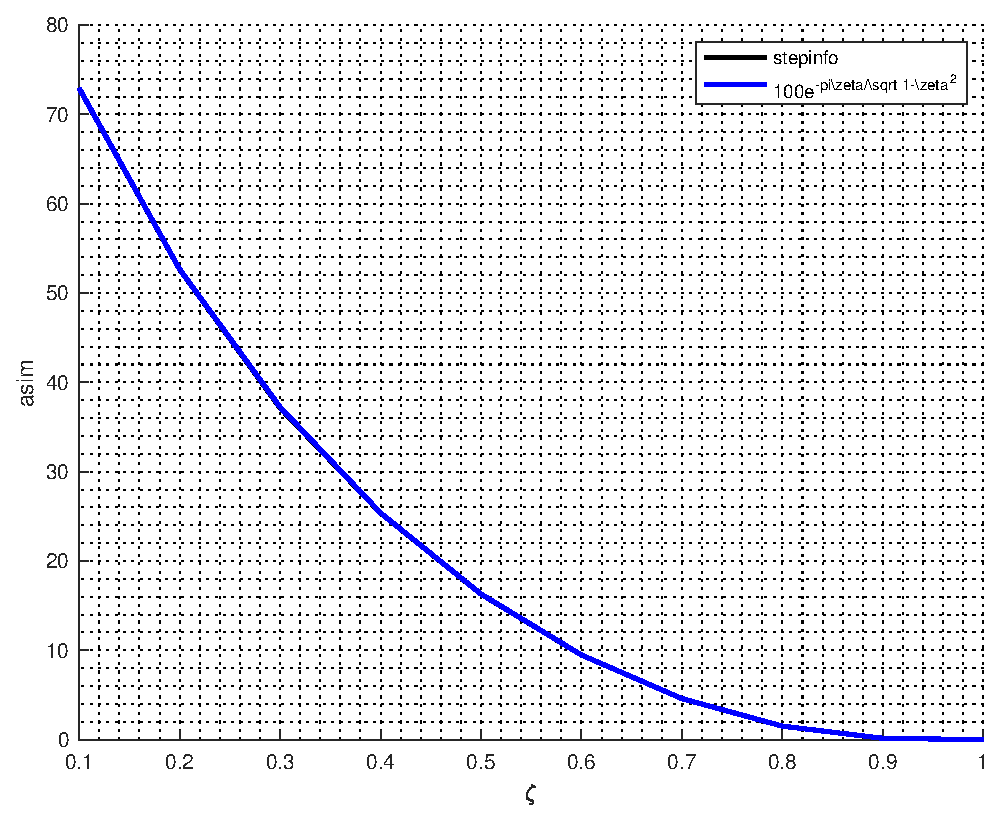
\includegraphics[width=0.5\textwidth]{img/lec4_plot4}
        \caption{Denklem~\ref{eqn:second_order} ile verilen sistem için aşım}
        \label{fig:lec4_plot4}
    \end{figure}
\end{enumerate}
% 1-exp(-4*t)*(cos(5.457*t)+0.733*sin(5.457*t))
